\documentclass[acmtocl,acmnow]{article}

%\newtheorem{theorem}{Theorem}[section]
%\newtheorem{conjecture}[theorem]{Conjecture}
%\newtheorem{corollary}[theorem]{Corollary}
%\newtheorem{proposition}[theorem]{Proposition}
%\newtheorem{lemma}[theorem]{Lemma}
%\newdef{definition}[theorem]{Definition}
%\newdef{remark}[theorem]{Remark}
\usepackage[utf8]{inputenc}
\usepackage{graphicx}
\def\firstfoot{\def\@firstfoot{}}
\def\runningfoot{\def\@runningfoot{}}
\usepackage{numprint}
\usepackage{cite}
\usepackage{hyperref}
           
\markboth{Florian Markowsky}{efficient storage of genome resequencing data}

\title{A novel compression tool for efficient storage of genome resequencing data}
            
\author{Florian Markowsky}
            
\begin{document}

 
%\begin{bottomstuff} 
%\ldots
%\end{bottomstuff}

\maketitle
\begin{minipage}{3cm}
  \begin{center}
    
\includegraphics[width=2cm]{img/ZBH_Logo_Neu.pdf}
  \end{center}
\end{minipage}
\begin{minipage}{6cm}
  Universität Hamburg\\
  Zentrum für Bioinformatik
\end{minipage}
\begin{minipage}{3cm}
  \begin{center}
    
\includegraphics[width=2cm]{img/UHH_Logo.pdf}
  \end{center}
\end{minipage}

\begin{abstract} 
  In this article, the storing problem of huge amounts of data resulting from modern sequencing technologies will be 
  discussed. Different approaches for efficient storage of large sequences will be introduced and the algorihm to
  compress genome resequencing data of \cite{WaZh} will be presented in detail. In the last section, possible
  future developments will be taken into account and a BLAST algorithm working directly on compressed data will be 
  presented.
\end{abstract}           

  
\tableofcontents

\newpage

\section{Introduction}

Next generation sequencing technologies have revolutionized the acquirement of genome sequence data. While it tool more
than ten years and $400.000.000$\$ to sequence the first almost complete human genome, it is now only a matter of about
one week and less than $1.000$\$(\cite{LohBamBer}). As it can be seen in \ref{gspp}, the problem that occurs is that the
amount of genome data outgrows the processing power since 2006. This means that to store the data emerging from
sequencing, the storage budgets of every sequence storing database has to increase every year. Sequence information
is just growing faster than available disk space.

This makes it more important than ever to have efficient compression techniques to store great amounts of sequencing data
on limited disk space. 
The first approach here would be to use standart compression techniques like \emph{LZ77} or \emph{gzip2}. These algorithms
use sliding windows to find repeats and compress by encoding this repeats instead of storing them more than once. These
algorithms however are not fit to deal with genome data, since genomes are on the scale of $10^5$ to $10^{10}$ base pairs
in animals. To compress sequences of that size with these standart approaches, multi-gigabyte buffers would be needed
(\cite{DeoGra}).
Special developed genome compression algorithms now also use the fact that there are many inter-genomic and intra-genomic
repeats, but are designed from the start to deal with huge amounts of data.

A single genome now contains much information, and although a certain degree of compression can be
achieved due to repeated regions, this is not comparable to the huge compression potential when many genomes of the same 
species are stored. Since these
genomes do not differ that much in general and differ only in about 1\% of bases in humans, the approach
to just store differences to a reference sequence seems to have promising potential for genome database space reduction 
(\cite{LohBamBer}).

\begin{figure}
  \begin{center}
    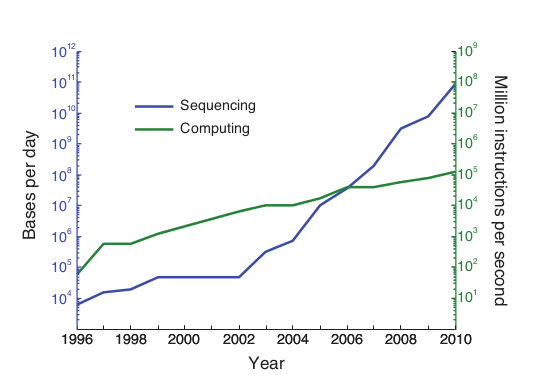
\includegraphics[height=0.3\textwidth]{img/Moorevsgen.png}
    \label{gspp}
    \caption{Growth of genomic sequence data compared to acceleration of processiong power according to Moore's Law
            , \cite{LohBamBer}.}
  \end{center}
\end{figure}

An appropriate compression algorithm for genomic data should satisfy certain demands.
The first and most important one obviously is to reduce file size as much as possible without the loss of any information.
Besides that, there are other optional qualities, making an algorithm more useable in practise. It is very desireable
that compression and decompression only takes a passable amount of time, since scientific workflows will not allow to wait
several hours for compression or decompression of genome data.
Furthermore, if many genmoic sequences are stored in one file, there should be no need to decompress the whole lot of 
sequeces if only one of them needs to be accessed. Some random access functionality or a partly decompression would come
be fitting to handle party of the big amounts of genomic data.

\section{Common techniques}

\subsection{Huffman-Coding}

\label{huff}
Huffman coding is a coding method presented by \cite{huff} in 1951, that encodes characters depending on the frequence 
of their occurence in a given string. The more frequent a character occurs, the shorter the corresponding code is.
It guarantees the smallest possible number of digits required to encode a string by
using variable length prefix free codes.

\subsection{Match finding}
\label{hash}

Since most compression algorithms for DNA data aim on storing only the differences of the input sequence in respect to a
reference sequence, the first task is to find these differences. This is analog to finding the matching
regions, since knowing them easily lets you find the differences. Seeing this, match finding becomes an important task in
compression.

Naive match finding computes an alignment of the two sequences, therefore taking $O(nm)$ time. When computing in genomic
scales, this is no option in terms of efficency. Hash arrays and Suffix trees have been used to avoid these high runtime
costs.

%TODO hash array match suche beschreiben

A Suffix trees is an index data structure... 
%TODO suffix array match suche beschreiben (GIK script)

\section{State of research: different compression techniques}

There have been many different approaches on the compression problem for genomic sequences. In this section, three
different approaches of 2011 will be presented. The first one will be a reference based compression (\cite{FriLeiCho}),
that compresses reads derived from next generations equencing technologies by aligning them to a reference sequence.
After that, an iterative dictionary construction algorithm (\cite{Kur}) will be preseneted, that compresses whole genome
sequences and, in contrast to all other
algorithms presented in this work, does not need any reference sequence to compress or decompress.
Next, a robust relative compression approach with random access (\cite{DeoGra}) is described, that stores whole genomes
as positions of matches with a reference sequence.

\subsection{Reference-based read compression}

The reference-based compression of \cite{FriLeiCho} stores short sequence reads that most next generation sequencing
technologies are producing. It does so by computing an alignment of the reads to a reference sequence and storing 
the relative starting position of every read, along with strand and indel information. This data is encoded using
Golomb-codes. Similar to Huffman-codes, Golomb codeing is a variable length coding scheme. If the data that is to encode
is nearly geometrical distributed, Golomb coding is just as efficient as Huffman, while using less memory (\cite{Gol}).

  \begin{figure}
\begin{center}
    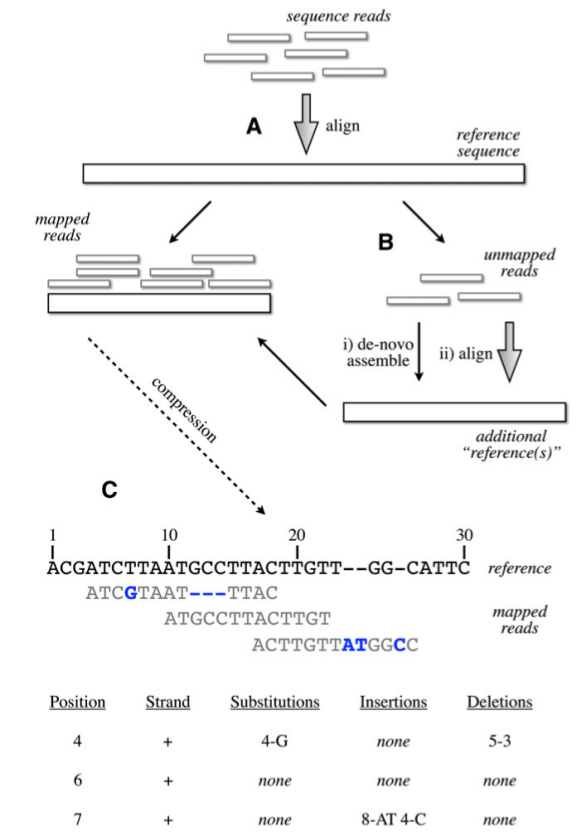
\includegraphics[height=\textwidth]{img/ReadCompressionSchematic.png}
    \label{readcomp}
    \caption{Schematic view of the reference-based read compression. In the first step (A), reads are aligned to the
    reference sequence. Reads that can not be mapped to the reference (B) are a major flaw of this approach. 
    (C) shows the alinment in detail. In the lower part, the store scheme is shown: along with the relative starting position,
    the strand the read is aligned to and information about positions of substitutions, insertions and deletions is stored.
    \cite{FriLeiCho}}
\end{center}
  \end{figure}

Problems occur if not all reads can be mapped successfully against the reference sequence. Unmapped reads cannot be stored
as match positions, and therefore can not be treated like the mapped reads. One option would be to just dicard them. But
this would mean a loss of information and therefore not be appropriate. in \cite{FriLeiCho}, it is proposed that the
unmapped reads should be pooled an an additional reference sequence shold be composed using sequence assembly methods 
(a deBruijn graph, in particular). The originial reference sequence qould be extended by the one generated in this way.
This increases the performance a little, but since the unmapped reads are not very suitable for assembly methods (e.g.
there might not be any overlaps) it is no optimal solution.

Anyway, the compression is more efficient than stadart compression techniques. As can be seen in table \ref{ReadComTab},
The human test genome NA12878 was encoded using $19.96$bpb in the FASTQ format, also storing base quality information,
and $11.45$bpb in raw FASTA. By using bzip2, a standart file compression algorithm, the genome could be compressed to
$6.64$bpb with quality information and $1.84$bpb without.
%TODO Discussion
\begin{table}
  \begin{center}
    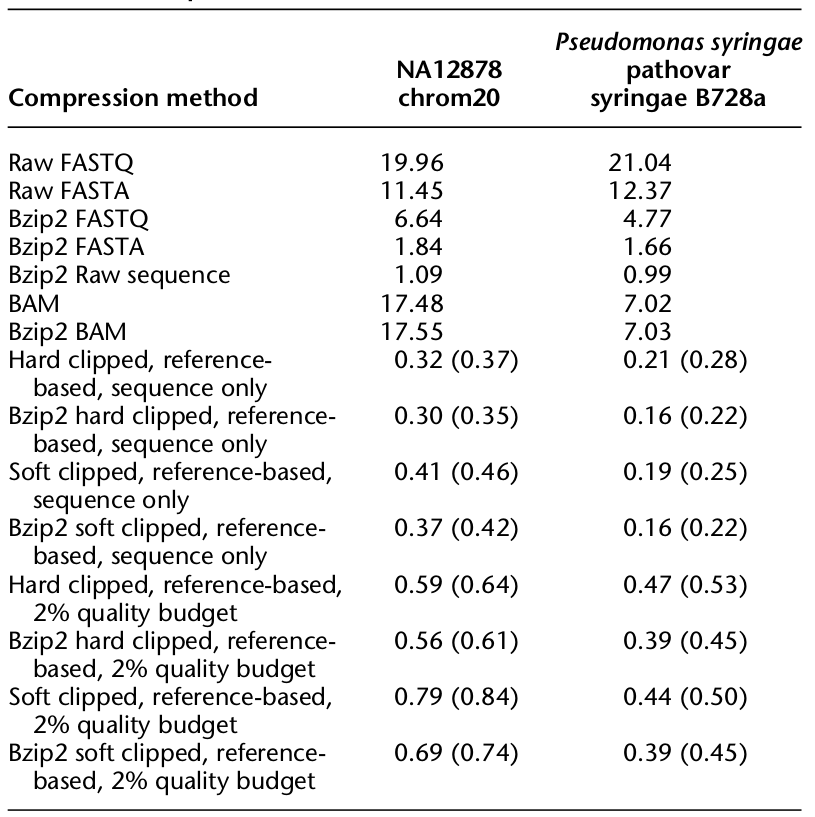
\includegraphics[width=\textwidth]{img/ReadCompTab.png}
    \label{ReadCompTab}
    \caption{The left column shows the data format, while the middle and right columns show the compressed sizes (in Bits 
    per Base) of human and bacterial genomic data, respectively. (\cite{FriLeiCho})}
  \end{center}
\end{table}
   % & reference based & raw FASTA & bzip2 \\
   % human genome & $0.41$ bpb & $11.45$ bpb & $1.84$ bpb \\
   % bacterial genome & $0.19$ bpb & $12.27$ bpb & $1.66$ bpb \\
Summing up, it can be said that the reference-based read compression approach achieves a $10$- to $30$-fold better
compression than standard compression  approaches.

\subsection{Iterative dictionary construction: COMRAD}

The COMRAD Algorithm, presented in \cite{Kur}, is an iterative dictionary construcion algorithm finding a gramar of the
sequences that are to be compressed. The compressed sequences consist of nonterminals representing parts of the input
according to the created gramar. The authors hope to achieve efficiency by replacing large or often occuring repeats 
with nonterminals, saving more space than the overhead to store the gramar costs. Since it is an NP-hard problem to find
the smalles gramar for a given language, this algorithm uses a greedy strategy to produce good results in reasonable time.

The algorithm works interative, so mutiple runs over the input data are necessary. Each iteration can be devided in two
steps. At first, a frequency
dictionary storing the freuqncy of all substrings of a given length is created. Then, all subsequences occuring more often
than a given threshold are replaced by a new nonterminal that is added to the dictionary. The reulst of each iteration is
a modified dictionary, the modified alphabet with the new nonterminals and the set of compressed sequences, where the
substrings have been replaced by the nonterminals. After the last iteration, these results are encoded using the
Huffman coding scheme.

Each iteration requires two passes over the input data. The number of iterations depends on the input size. It can 
roughly be said that the number of iterations grows by one or two per decimal order of magnitude of input growth (
\cite{Kur}). The first step of each iteration takes $O(n)$ time, while the substitution takes $O(n \log n)$.

  \begin{figure}
\begin{center}
    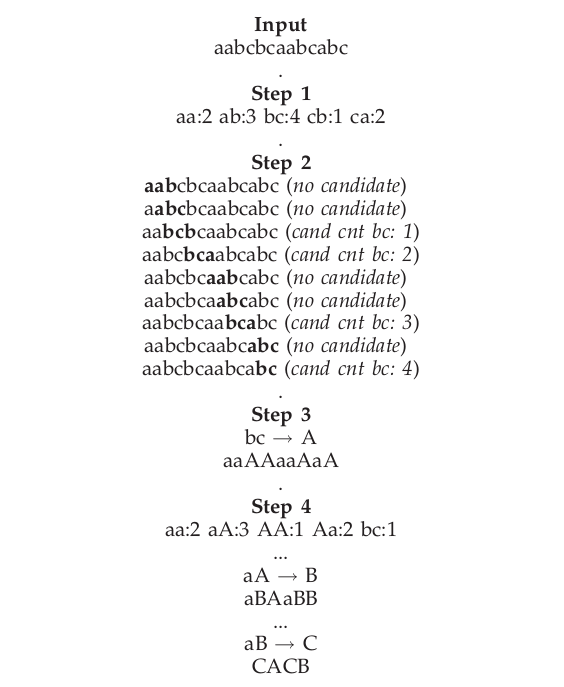
\includegraphics[height=\textwidth]{img/Comrad.png}
    \label{comrad}
    \caption{Compression with RAY}
    %Parameters: length L of substrings for first iteration (default: 16), 
    %frequency F(default:4): when to take words in dictionary
    %in consecutive runs, only sequences with nonterminal symbols must be considered 
    %(in certain patterns)
\end{center}
  \end{figure}
In figure \ref{comrad}, the workflow of the RAY algorithm, on which COMRAD is based, is shown to visualize the 
encoding principles. In the first step, the quantities of substrings of a certain length $k$ (in this case: two)
are stored in the frequency dictionary. All substrings which count exceed a certain threshold are considered 
potential substitution candidates. Next, all substrings of length $k+1$ are scanned. If the frequency dictionary
count of the leftmost $k$word is higher than the one of the rightmost one, the candidate count is incremented.
This procedure ensures that the substitution of one substring does not hinder the substitiution of a more frequent one.
In the third step, a new replacement entry is created in the dictionary and the substitution of all occurences of the
substring is performed. This is continued until no more substitutions can be made.
%TODO verifizieren

COMRAD provides random access on the compressed sequences, since when the start- and end positions of a fragment is 
known, it can be reconstructed using the dictioary. It is obvious that the efficiency of this approach increases with more
and longer repeats and therefore with increasing data size and an increasing number of sequences to be compressed.
Contrary, it has nearly no effect on small datasets with few and short repeats, since the disproportional large codebook
outweights the storage cost savings.

Table \ref{comreadRes} shows the compression results of mutiple genomes using the COMRAD algorithm. Some results are quite
efficient, e.g. compressing Influenza genomes from $1.97$bpb to $0.43$bpb. The compression of the human genome however is
very unsatisfactory, since compressing to $1.44$bpb can nearly be achieved by standart compression approaches (see 
\ref{ReadCompTab}).
The authors claim that the bad results are due to the small number of human genomes available to that time. Since they
used only four genomes, the created codebook war disproportionaly large, since there were to few and to short repeats.
To prove this, the authors generated artificial chromosome 22, chromosome 1 and chromosome 20-datasets, using two
real chromosomes as parents and iteratively joining and mutating them. In the chromosome 1-case, $127$ sequences were
generated and compressed to $0.07$bpb. This is quite an efficient compression, but should be considered carefully since
not derived from real data.

Compression time on large datasets are up to $8$hrs in the four human genome case, which means just about $0.42$MB/s, and
up to $49$hrs in the artificial
human chromosome case. This can be seen as a major flaw of this technique, since there are much faster compression
algorithms with equal or better compression results.

\begin{table}
  \begin{center}
    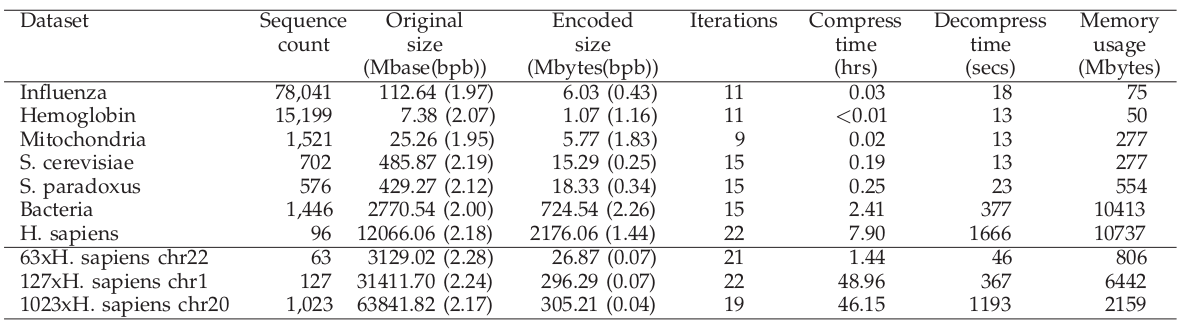
\includegraphics[width=1.2\textwidth]{img/comradRes.png}
    \label{ComradRes}
    \caption{Compression results of the COMRAD algorithm for different data sets. (\cite{Kur})}
  \end{center}
\end{table}

%    \item Influenza genomes $113$ MB ($1.97$ bpb) to $6$ MB ($0.43$ bpb)
%    \begin{itemize}
%      \item time for compression: about $0.03$h $\rightarrow$ $1.04$ MB/s
%    \end{itemize}
      %time: 0.03h
%    \item Yeast genomes $485.87$ MB ($2.19$ bpb) to $15.29$ MB ($0.25$ bpb)
%    \begin{itemize}
%      \item time for compression: about $0.19$h $\rightarrow$ $0.71$ MB/s
%    \end{itemize}
      %time: 0.19
%    \item 4 human genomes \numprint{12066.06} MB ($2.18$ bpb) to \numprint{2176.06}MB ($1.44$ bpb)
%    \begin{itemize}
%      \item time for compression: about $8$h $\rightarrow$ $0.42$ MB/s
%    \end{itemize}
    %problem: codebook very large -> better when compressing bigger number of genomes:
    %   artificial generated human dna compressed to 0.07bpb (31.41gb to 0.29gb)
%  \end{itemize}

\subsection{Robust relative compression with random access}%TODO präziser ausführen?
\label{GDC}

In \cite{DeoGra}, the relative compression tool Genome Differential Compressor (GDC) is presented that parses an 
input sequence, one or several genome sequences, into a sequence of matches and literals.
As described in section \ref{hash}, a  hash array is used to find matches. These matches are stored as a pair of reference
offset and match length. To provide random access, the algorithm works blockwise. That means that the reference offset is
stored with respect to the starting position of the last block, which also leads to smaller offset numbers that can be
stored more efficiently using Huffman coding.
Instead of greedy picking of the first match, a dynamical-sized lookahead buffer is used to
determine whether a match starting in one of the following position might be better. A better hit here must not always 
mean a longer hit, since smaller ones may be favoured if their offset can be stored cheaper.
Literals are stored by packing them in supersymbols as far as it is possible and also encode them using Huffman. %TODO supersymbols?
The reference sequence is stored in the same way, creating overhead that is significant in small datasets but is not so
important in bigger ones.

\begin{table}
  \begin{center}
    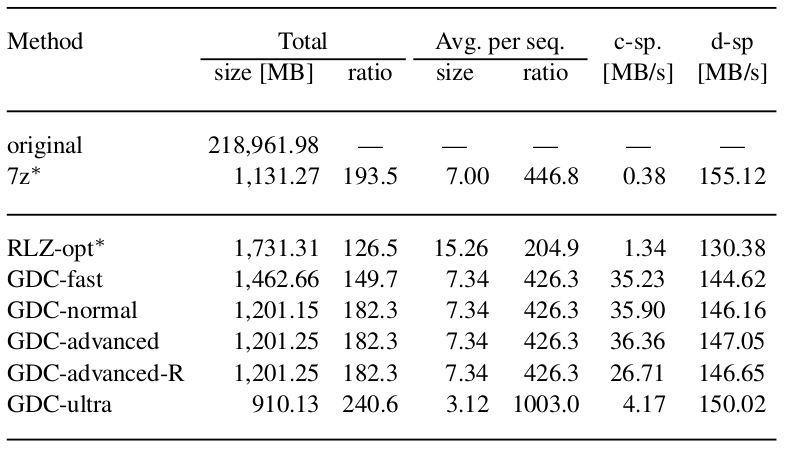
\includegraphics[width=1\textwidth]{img/DeoGraRes.png}
    \label{DeoGraRes}
    \caption{Compression results of different GDC variants on a set of $70$ human genomes. (\cite{Kur})}
  \end{center}
\end{table}

As mentioned above, random access is possible due to blockwise encoding.
In table \ref{DeoGraRes}, compression results of the different variants of GDC in comparison 7zip and 
RLZ-opt are shown when compressing $70$ human genomes, summing up to \numprint{218 961.98}MB of data.
It can be seen that GDC performs an effective compression, reducing the file size to \numprint{1 201.15}MB. With 
compression speed of $36.36$MB/s, it is also by far the fastest compression algorithm presented here so far.

\section{Genome ReSequencing tool}

The Genome ReSequencing tool is presented in \cite{WaZh}. It performs a chromosome-wise compression of a given iput
chromosome set with respect to a reference chromosome set. The result is a difference file containing the discrepancy from
the reference sequence and a command file that is used to decompress the difference file back to the original input 
sequence.

The algorithms starts by computing the varied sequence percentage $\delta$. Depending on this, the algorithm either breaks,
if $\delta$ is bigger than $0.1$, because the data is too different from the input set to be compressed efficiently,
or, if $\delta$ is between $0.1$ and $0.03$, the chromosome is cut into $n$ pieces. These pieces are aligned to the reference
chromosome, testing different cut positions, %TODO nochmal nachlesen: zerschneiden?!
until the sum of the $\delta_i$ for each piece is minimized.
If $\delta$ is smaller than $0.03$, the main part of the algorithm starts to compute the difference file.

To compute the difference file, the longest common local nucleotide sequence is computed. The method is demonstated in
figure \ref{ComSubProc}. For every symbol in sequence X, every occurence in Y is marked. A path through the marked positions
is searched, which represents the longest common local nucleotide sequence.
The computation mathed is similar to the UNIX diff program, and a similar file is produced. This file is further processed
into the final difference file. The procession steps can be seen in figure \ref{ComSubProc}.

Part a shows the output generated by the diff program. Each entry consists of one line saying which lines of the first file
hast been modified in which way to which lines of the second file. Possible modifications are additions ('a'), deletions
('d') and changes ('c'). Then in case of an addition, the added lines are shown, for a deletion the deleted lines, and 
for a change the removed and the newly added lines. The first procession step changes the operation codes from a, d, c to
i, d, h and removes redundant information: since we know the reference sequence and the position in the reference file,
there is no need to store which bases we delete. The same applies for the bases deleted when changed.
In the last step, tabulators are inserted to make the file better machine-readable and the position information is
changed to a relative representation, so smaller numbers have to be stored.
Finally, the difference file is Huffman encoded.

%TODO Grafiken nebeneinander
\begin{figure}
\begin{minipage}{5cm}
    \begin{center}
      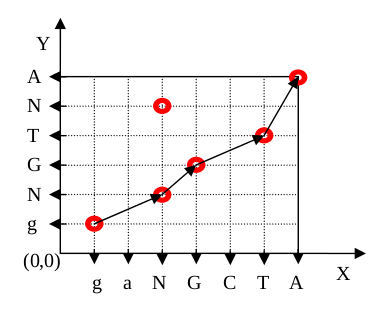
\includegraphics[height=\textwidth]{img/WaZhComSub.png}
    \end{center}
\end{minipage}
\begin{minipage}{5cm}
    \begin{center}
      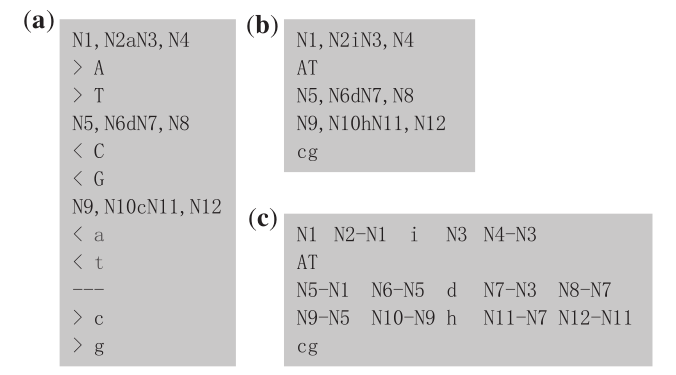
\includegraphics[height=\textwidth]{img/WaZh2.png}
      %a. raw changes generated by diff
      %b. stripped of redundant information: does not matter WHAT was deleted
      %   bei ersetzungen egal was ersetzt wurde
      %c. relative Positionsangaben
    \end{center}
\end{minipage}
\label{ComSubProc}
\caption{Left: Computation of the longest common sequence. Right: Procession steps of the difference file: a: generated 
          diff file, b: redundancys removed, operation codes changed, c: /t added, relative postitions. \cite{WaZh}}
\end{figure}

\begin{figure}
  \begin{center}
    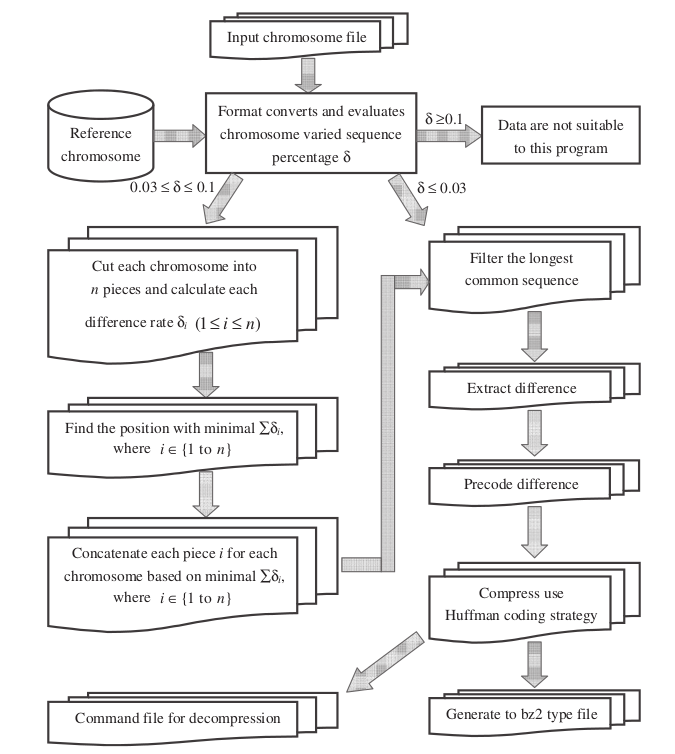
\includegraphics[width=\textwidth]{img/WaZh.png}
    \label{WaZhStructure}
    \caption{Structure of the GRS tool. \cite{WaZh}}
  \end{center}
\end{figure}

The GRS tool allows effective compression. Rice genomes of a total size of $361$ MB were compressed to $4.4$ MB at a
rate of $0.26$ MB/s. A human genome was compressed from  \numprint{2986.8}MB to $18.8$ MB at a rate of $1.81$ MB/s. 
The grade of compression is satisfactory, but in terms of speed the GDC algorithm is much faster, although GRS is still
faster than COMRAD. A random access is not mentioned by the authors. It is not possible in this approach, since positions
are stored relative but not blockwise, so the whole chromosome sequence represented by the difference file has to be
compressed.

\section{Future development}

All the presented algorithms satisfy our demands for effective compression of genomic data. The basic problem of available
disc space can be resolved, especially the GDC algorithm (section \ref{GDC}) is also efficient in terms of  compression
speed.

However, a flaw all the presented algorithm share with most other algorithms found in literature is the need to decompress
all the data or all the parts of the data on which computations are to be made. An aim for future development should
be the development of algorithms that directly work on compressed data. Such an algorithm taken from \cite{LohBamBer}, where
it was implemented as a proof of concept, will now be presented.

\subsection{CaBLAST}

The Compression accelerated BLAST algorithm is an improvement of the well known BLAST algorithm. The authors decided to
use BLAST as underlying search tool because of its vast application and its status as de-facto standart sequence search
algorithm.

The Algorithm works in two steps: a preprocession, that is in fact the compression of the input data, and the CaBLAST
algorithm itself. In the preprocession, an unique database is constructed, containing all unique substrings from the 
input sequence database. Repetitions in the original database are stored as pointers from the fist occurence of the
substring in the unique database to the starting point of the repetition. These pointers are stored in the link table.
The repetitions do not have to be perfect hits, a certain amount of mismatches is allowed.

The CaBLAST algorithm performs a search in two stept: The BLAST search at first is performed as a coarse search with
relaxed thershold on the unique database. All repetitions of the Hits found are looked up in the link table, the links 
are traced and a fine BLAST with the opriginal threshold is performed on the hits of the first run and the repetitions 
traced by the link table.
Figure \ref{CaBLAST} gives an overwiew over the preprocessing as well as the CaLAST search.

\begin{center}
  \begin{figure}
    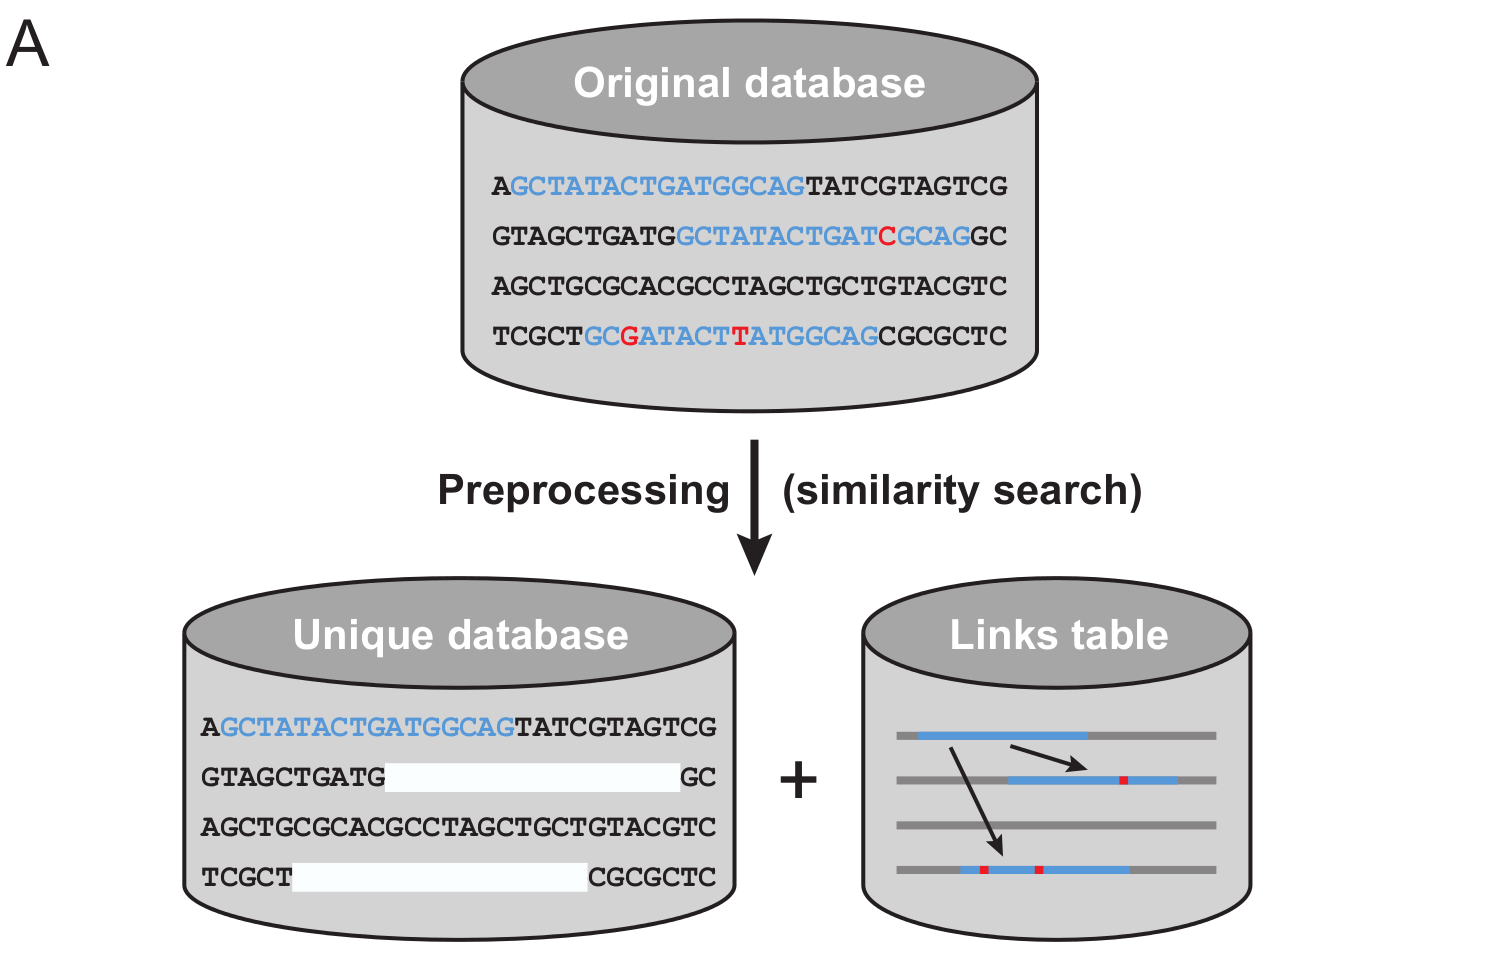
\includegraphics[width=\textwidth]{img/Compgenp1.png}
    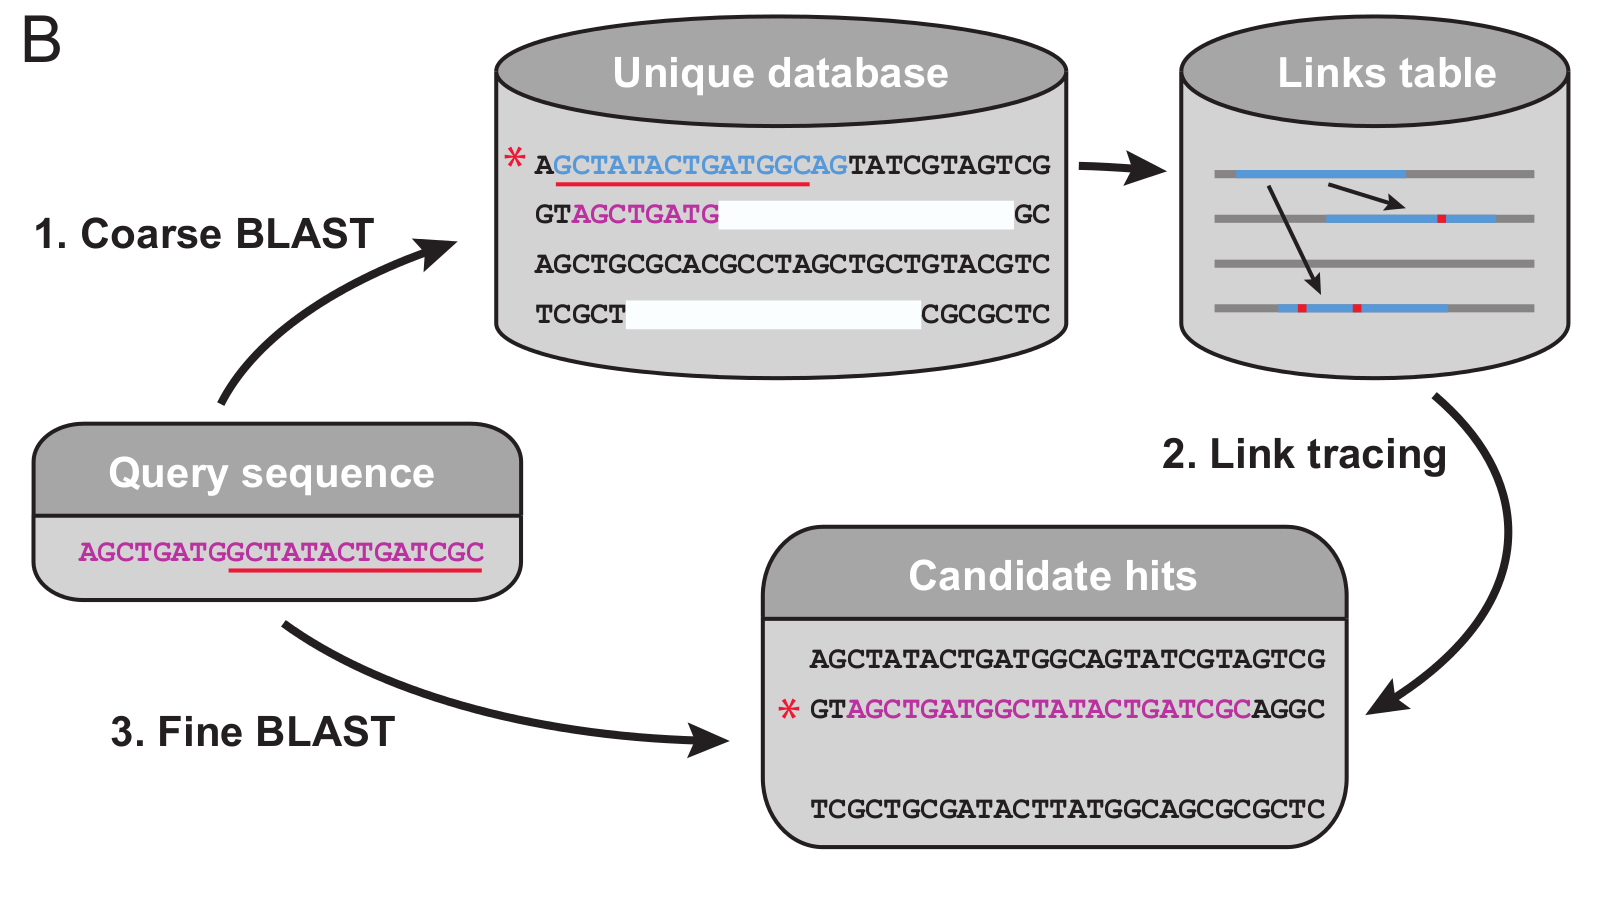
\includegraphics[width=\textwidth]{img/Compgenp2.png}
    \label{CaBLAST}
    \caption{A: preprocession for CaBLAST: the input database is divided in an unique database
    and a link table. B: CaBLAST algorithm: a coarse BLAST is performed on the unique database. Links are traced and a
    fine BLAST is performed on the original hits and the traced links. \cite{LohBamBer}}
  \end{figure}
  \end{center}
  
The runtime of the preprocessing is linear to quadratic, but only has to be performed once for a database. The place needed
for the storage of the databased is of course reduced drastcally. But since the 
amount of data the coarse BLAST search has to search is reduced alike, the overall runtime is much lower than the one
of the original BLAST on the unprocessed input database.

\begin{figure}
  \begin{center}
      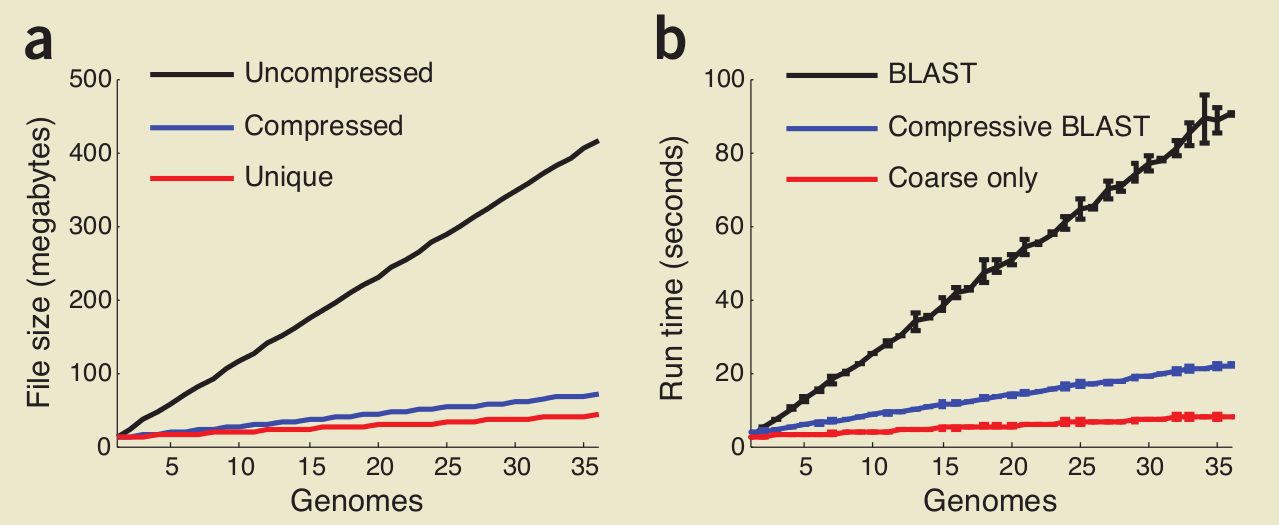
\includegraphics[width=\textwidth]{img/CaBLASTrtfs.png}
      \label{CaRes}
      \caption{Results of the CaBLAST algorithm: Space requirements as well as runtime is significantly lower than the 
      usual BLAST approach. \cite{LohBamBer}}
  \end{center}
\end{figure}

%TODO Fazit

%Bibliography
\newpage
\small
\bibliographystyle{unsrt}    
\bibliography{quellen}

\end{document}
